\textbf{Цель работы:} изучение вольт-амперной характеристики нормального тлеющего разряда; исследование релаксационного генератора на стабилитроне. \\

\textbf{Используемое оборудование:} стабилитрон СГ-2 (газонаполненный диод) на монтажной панели, магазин ёмкостей, магазин сопротивлений, источник питания, амперметр, вольтметр, осциллограф.
                    
\section{Теоретическое введение}

Принципиальная схема релаксационного генератора, представляющего собой электрический контур, состоящий из ёмкости $C$, резистора $R$ и газоразрядного диода с $S$-образной вольт-амперной характеристикой, изображёна на рис. 1. Релаксационные колебания в этом
случае являются совокупностью двух апериодических процессов -- зарядки конденсатора и его разрядки. В рассматриваемой установке роль «ключа», обеспечивающего попеременную зарядку и разрядку конденсатора, играет газоразрядный диод.

\begin{figure}[h]
    \centering
    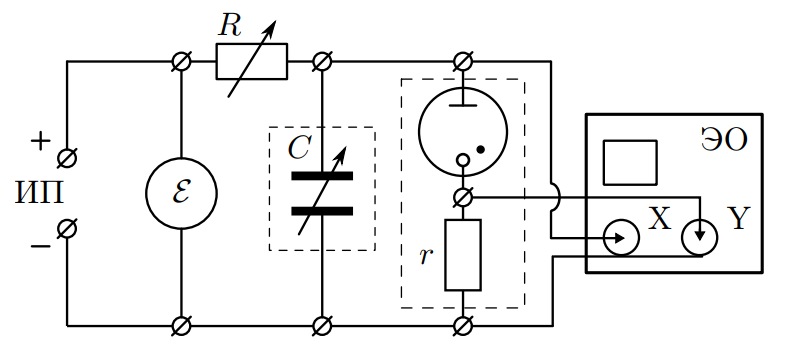
\includegraphics[width = 10 cm]{images/1.png}
    \caption{Cхема релаксационного генератора}
    \label{p1}
\end{figure}

Зависимость тока от напряжения для газоразрядной лампы не подчиняется закону Ома и характеризуется рядом особенностей, представленных в упрощённом виде на рис. 2 вместе с нагрузочной прямой $I = I_0 \left( 1 - U / \varepsilon \right)$, где $\varepsilon$ — постоянное напряжение внешнего источника
питания.

\begin{figure}[h]
    \centering
    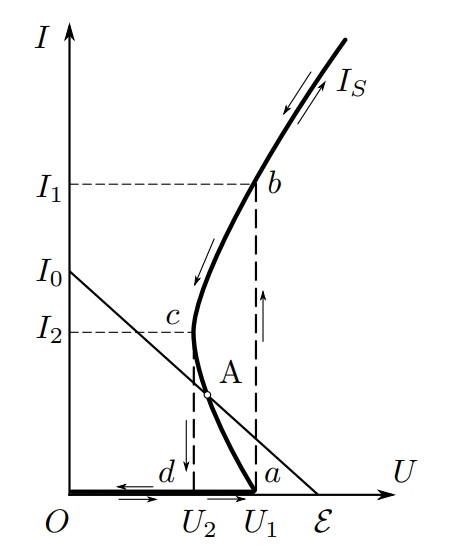
\includegraphics[width = 6 cm]{images/2.png}
    \caption{Упрощённая вольт-амперная характеристика стабилитрона}
    \label{p2}
\end{figure}

Ток в лампе возникает только в том случае, если разность потенциалов на её электродах достигает напряжения зажигания $U_1$. При этом скачком (участок $ab$) устанавливается конечная сила тока $I_1$ -- в лампе возникает нормальный тлеющий разряд. При дальнейшем незначительном увеличении напряжения сила тока заметно возрастает по закону, близкому к линейному.

Если начать уменьшать напряжение на горящей лампе, то при напряжении $U_1$ лампа ещё не гаснет, и сила тока продолжает уменьшаться
(участок $bc$ на рис. 2). Лампа перестаёт пропускать ток лишь при напряжении гашения $U_2$, которое обычно существенно меньше $U_1$. Сила тока
при этом скачком падает от значения $I_2 < I_1$ до нуля (участок $cd$).

В стационарном режиме, когда напряжение $U$ на конденсаторе постоянно и $dU/dt$ = 0, ток через лампу равен

\begin{equation}
    I_{\text{ст}} = \frac{\varepsilon - U}{R + r}
\end{equation}

При этом возбуждение автоколебаний возможно только при выполнении условия

\begin{equation}
    R + r < - \frac{1}{I'_S(U_A)}
\end{equation}

При зарядке конденсатора через сопротивление $R$ напряжение на нём увеличивается (рис. 3). Как только оно достигнет напряжения зажигания $U_1$, лампа начинает проводить ток, причём прохождение тока сопровождается разрядкой конденсатора. В самом деле, батарея $\varepsilon$, подключённая
через большое сопротивление $R$, не может поддерживать необходимую для горения лампы величину тока. Во время горения лампы конденсатор разряжается, и когда напряжение на нём достигнет потенциала гашения $U_2$, лампа перестанет проводить ток, а конденсатор вновь начнёт заряжаться. Возникают релаксационные колебания с амплитудой $U_1 - U_2$.

Полное время одного периода колебаний $T$ состоит из суммы времени зарядки $\tau_{\text{з}}$ и времени разрядки $\tau_{\text{р}}$.
Однако если сопротивление $R$ существенно превосходит сопротивление
зажжённой лампы, то $ \tau_{\text{з}} \gg \tau_{\text{р}}$ и $T \cong \tau_{\text{з}}$, что подтверждается в нашем эксперименте. Во время зарядки конденсатора лампа не горит ($I(U) = 0$,
и уравнение цепи приобретает вид

\begin{equation}
    RC \frac{dU}{dt} = \varepsilon - U
\end{equation}

Результат этого уравнения с учётом начальных условий имеет вид

\begin{equation}
    T \cong \tau_{\text{з}} = RC \ln{\frac{\varepsilon - U_2}{\varepsilon - U_1}}
\end{equation}

Развитая выше теория является приближенной. Ряд принятых при расчётах упрощающих предположений оговорён в тексте. Следует иметь в виду, что мы полностью пренебрегли паразитными ёмкостями и индуктивностями схемы. Не рассматривались также процессы развития разряда и деионизация при гашении. Поэтому теория справедлива лишь в тех случаях, когда в схеме установлена достаточно большая ёмкость и когда период колебаний существенно больше времени развития разряда и времени деионизации (практически $\cong 10$ с).

\section{Ход работы}
\subsection{Характеристика стабилитрона}

Установка со стабилитроном имеет встроенное сопротивление $r = 5,4$ кОм.

С помощью приведённой ниже схемы можно получить ВАХ стабилитрона, в частности измерить напряжения зажигания и гашения (с учётом петли Гистерезиса).

\begin{figure}[h!]
    \centering
    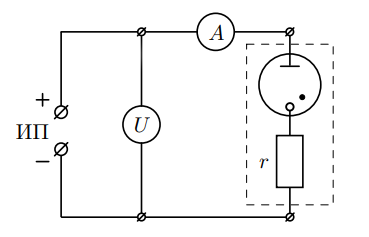
\includegraphics[width = 8 cm]{images/3.png}
    \caption{}
    \label{}
\end{figure}

Для этого снимем часть данных с приборов для построения ВАХ:

\begin{figure}[h!]
    \centering
    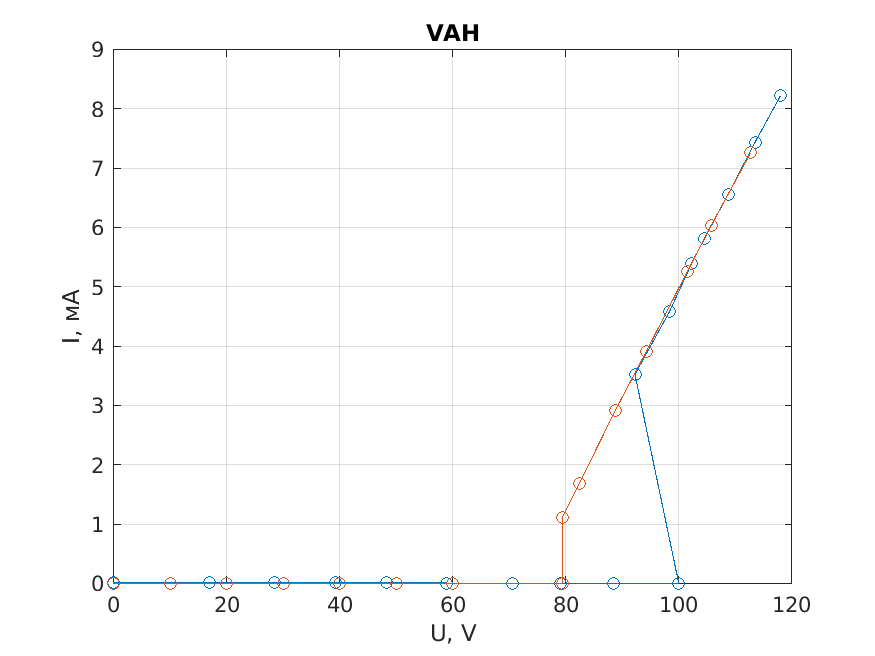
\includegraphics[width = 10 cm]{images/VAH.png}
    \caption{ВАХ стабилитрона}
    \label{vah}
\end{figure}

Здесь синяя кривая отвечает за увеличение напряжения, а оранжевая за уменьшение (рис. 4).

При этом график ВАХ стабилитрона без встроенного резистора имеет немного другой вид:

\begin{figure}[h!]
    \centering
    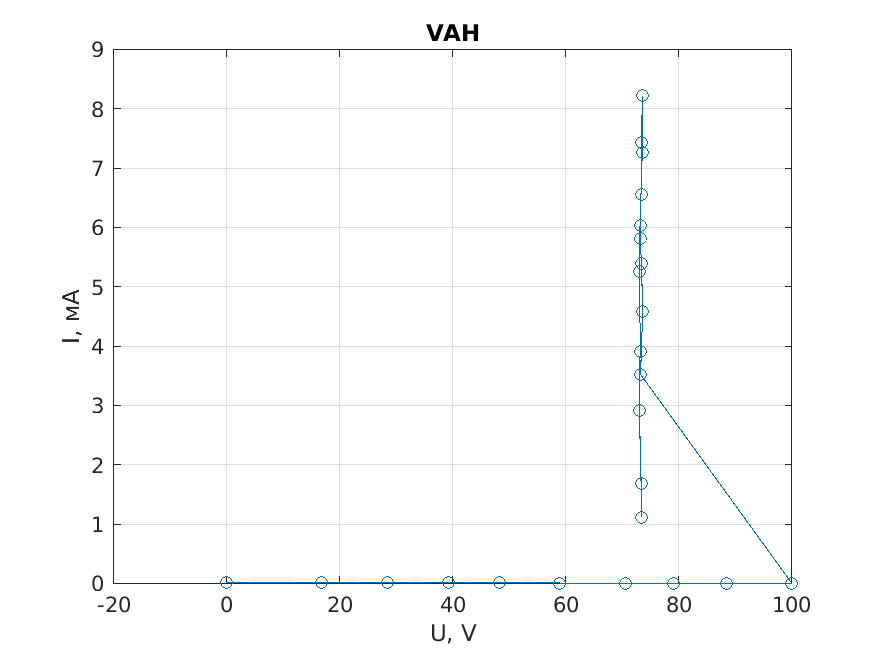
\includegraphics[width = 10 cm]{images/VAH2.png}
    \caption{ВАХ стабилитрона без учёта резистора}
    \label{vah2}
\end{figure}


Видно, что график вышел схожим по своей сути с теоретическим графиком.
Из него можно оценить напряжения зажигания и гашения, но для более точных значений проведём для этого несколько экспериментов и посчитаем среднее значение:

\begin{table}[h]
    \centering
    \begin{tabular}{|c|c|c|c|c|c|}
        \hline
        \textbf{$U_1, В$}  & 99,70 & 100,3  & 101,1  & 99,70 & 99,70 \\ \hline
        \textbf{$U_2, В$}  & 75,27 & 73,98  & 74,78  & 74,89 & 75,01 \\ \hline
        \textbf{$I_1, мА$} & 3,387 & 3,354  & 3,415  & 3,449 & 3,432 \\ \hline
        \textbf{$I_2, мА$} & 0,427 & 0,410  & 0,408  & 0,394 & 0,414 \\ \hline
    \end{tabular}
    \caption{Значения зажигания и гашения}
\end{table}

Итого имеем:

\begin{equation}
    U_1 = 100,1 \text{В}, \; \Delta  U_1 = 1,08 \text{В}
\end{equation}

\begin{equation}
    U_2 = 74,79 \text{В}, \; \Delta  U_2 = 0,95 \text{В}
\end{equation}

\begin{equation}
    I_1 = 3,407 \text{мA}, \; \Delta  I_1 = 0,058 \text{мA}
\end{equation}

\begin{equation}
    I_2 = 0,411 \text{мA}, \; \Delta  I_2 = 0,032 \text{мA}
\end{equation}

Погрешности были найдены через стандартное отклонение (среднеквадратичное значение) и являются погрешностями отдельного измерения. Также было учтено, что в статическом режиме измерения значение напряжения колебалось в пределах $0,46$ В, а значение силы тока в пределах $0,021$ мА.

\subsection{Времена гашения и зажигания}

Собрав схему, изоюражённую на рис. 1, установим сопротивление реостата $R = 900$ кОм, а ёмкость конденсатора $50$ нФ. Установив выходное напряжение источника питания $\varepsilon = 121 \pm 1$ В, установим по осциллограмме значения времён зарядки и разрядки:

\begin{equation}
    \tau_{\text{з}} = 39,5 \pm 0,5 \; \text{мс}
\end{equation}

\begin{equation}
    \tau_{\text{р}} = 0,65 \pm 0,05 \; \text{мс}
\end{equation}

Погрешности были учтены с помощью цены деления экрана осциллографа (в зависимости от масштаба развёртки -- $5$ $\text{ms/div}$ и $0,5$ $\text{ms/div}$ -- половина цены деления).

Для отношения времён имеем

\begin{equation}
    \frac{\tau_{\text{з}}}{\tau_{\text{р}}} = 60,7 \pm 1,2
\end{equation}

Очевидно, что суммарное время практически совпадает со значением времени зарядки $T = 40,15 \pm 0,55$ мс (погрешность посчитана по формуле косвенной погрешности через частные производные).

\subsection{Критический случай}

Определим критическое сопротивление реостата, при котором пропадают колебания в цепи: $R_{\text{крит}} = 138 \pm 1$ кОм.

При этом если сохранять значение сопротивления постоянным, а менять (уменьшать) значение исходного напряжения источника, то колебания тоже проадают при достижении некоторого значения.

\subsection{Исследование зависимости периода колебания цепи от её параметров}

Зафиксируем сопротивление реостата $R = 300$ кОм, вычислим, как зависит период колебания цепи от ёмкости конденсатора. В этом случае напряжение источника держим постоянным.
Зафиксировов экспериментальные значения и посчитав нужные теоретические значения, строим график.

\begin{figure}[h]
    \centering
    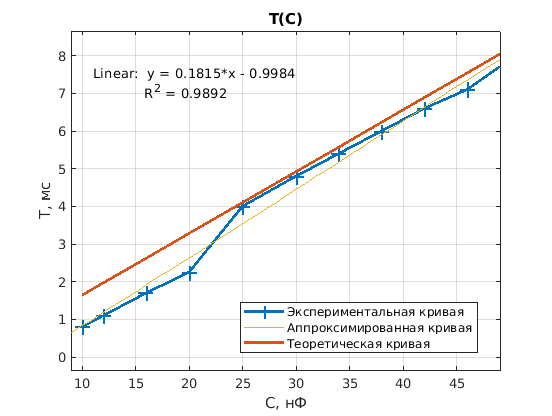
\includegraphics[width = 10 cm]{images/TC.png}
    \caption{Зависимость $T(C)$}
    \label{TC}
\end{figure}

\begin{figure}[h]
    \centering
    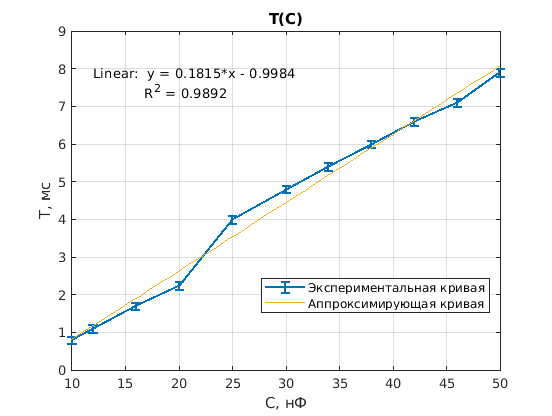
\includegraphics[width = 10 cm]{images/TC2.png}
    \caption{Зависимость $T(C)$ с ошибками измерения}
    \label{TC2}
\end{figure}

Видно, что вблизи центра рассмотренного набора значений графики почти совпадают, но на более низких ёмокстях происходит некоторый резкий спад периода. Возможно, он обсуловлен неточностью осциллографа. Значения ниже $10$ нФ не были рассмотрены, так как уже на этом этапе амплитуда колебаний на осциллографе заметно падает (вплоть до прекращения автоколебаний).

Для теоретической кривой коэффициент наклона равен $k = 0,158 \cdot 10^6$ с/Ф, для экспериментальной $(0,182 \pm 0,012) \cdot 10^6$ с/Ф. Значения различаются даже с учётом погрешности. В этом случае посчитаем динамический потенциал гашения $U_2$, воспользовавшись экспериментальной кривой и формулой:

\begin{equation}
    T = RC \ln{\frac{\varepsilon - U_2}{\varepsilon - U_1}} \Rightarrow U_2 = 82,3 \; \text{В}, \; \Delta U_2 = 2,1 \; \text{В}
\end{equation}

Погрешности для значения динамического потенциала гашения были найдены с помощью погрешности измерения $\varepsilon$, $k$ и стандартной формулы для погрешностей косвенных измерений.

Далее фиксируем ёмкость конденсатора $C = 50$ нФ, напряжение источника то же, что и было. Исследуем зависимость $T(R)$.

\begin{figure}[h!]
    \centering
    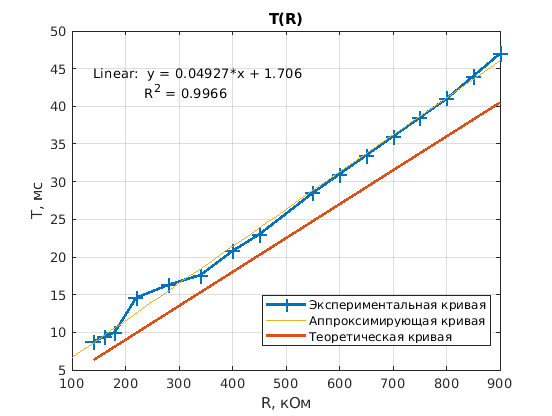
\includegraphics[width = 10 cm]{images/TR.png}
    \caption{Зависимость $T(R)$}
    \label{TR}
\end{figure}

\begin{figure}[h!]
    \centering
    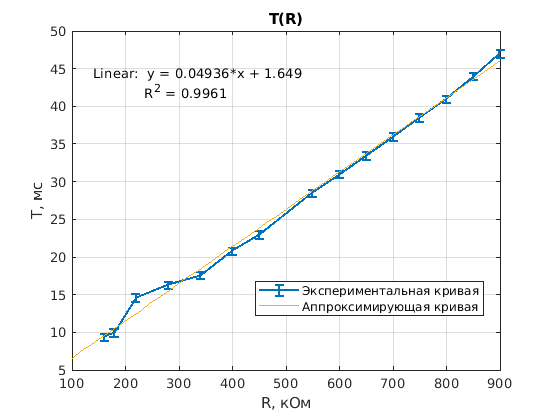
\includegraphics[width = 10 cm]{images/TR2.png}
    \caption{Зависимость $T(R)$ с ошибками измерения}
    \label{TR2}
\end{figure}

Видны флуктуации от прямой линии в районе $300$ кОм, которые не влияют на общий характер зависимости. Опять же, экспериментальная кривая почти совпадает с теоретической (характер зависимостей одинаков).

Для теоретической кривой коэффициент наклона равен $k = 44,5 \cdot 10^{-9}$ с/Ом, для экспериментальной $(49,3 \pm 2,1) \cdot 10^{-9}$ с/Ом. Значения аналогично различаются даже с учётом погрешности, как и для предыдущей зависимости. Посчитаем динамический потенциал гашения $U_2$:

\begin{equation}
    T = RC \ln{\frac{\varepsilon - U_2}{\varepsilon - U_1}} \Rightarrow U_2 = 84,8 \; \text{В}, \; \Delta U_2 = 1,7 \; \text{В}
\end{equation}

\subsection{Фазовые траектории релаксационных колебаний}

Установим параметры цепи $R = 900$ кОм, $C = 50$ нФ. Подключим генератор к осциллографу способом, указанном на рис. 8.

\begin{figure}[h!]
    \centering
    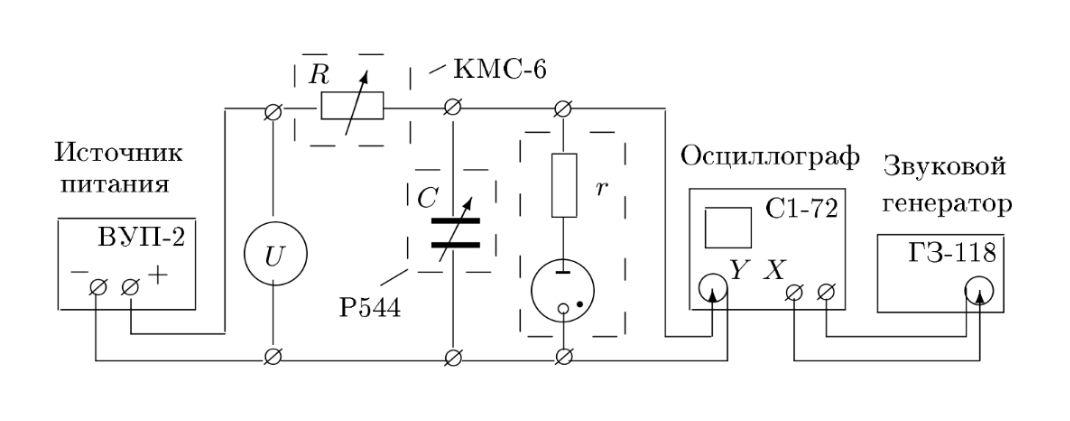
\includegraphics[width = 13 cm]{images/4.png}
    \caption{Схема подключение генератора}
    \label{gen}
\end{figure}

Установим по осям координат сдвиги и коэффициенты усиления, подходящие для наблюдения фазовой траектории релаксационных колебаний. 

Получим с помощью генератора фигуру Лиссажу 1:1, при этом с помощью фигур Лиссажу можно измерять частоту автоколебаний (через количество пересечений прямой линии -- свойства фигур Лиссажу).

\begin{figure}[h!]
    \centering
    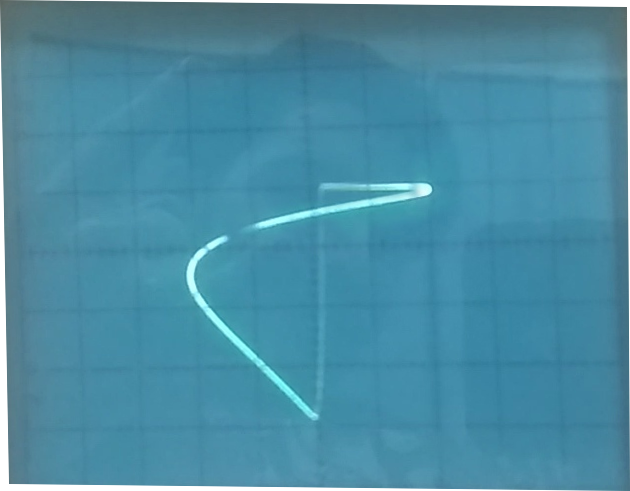
\includegraphics[width = 10 cm]{images/liss1.png}
    \caption{Фигура Лиссажу 1:1}
    \label{liss1}
\end{figure}

Аналогично получим фигуру Лиссажу для соотношения 1:2.

\begin{figure}[h!]
    \centering
    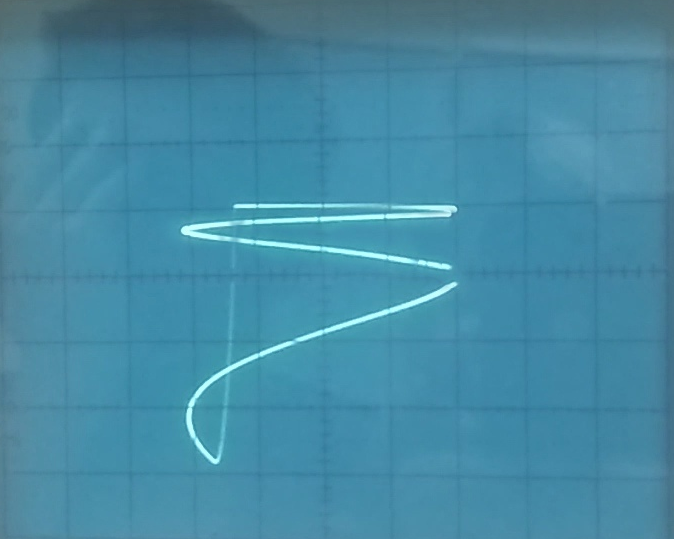
\includegraphics[width = 10 cm]{images/liss2.png}
    \caption{Фигура Лиссажу 1:2}
    \label{liss2}
\end{figure}

\section{Заключение}

Были найдены знчения напряжения и силы тока для зажигания и гашения для стабилитрона. 

С помощью осциллографа были найдены значения времён автоколебаний (в том числе отдельно для зажигания и гашения), в том числе зависимость времени автоколебания от ёмкости или сопротивления реостата в схеме.

Также частота могла быть найдена через фигуры Лиссажу, но в этом случае затруднительно найти отношения времён зажигания и гашения стабилитрона.


























